\section{Algebraic Moment Closures}
\label{sec:algebraicClosure}

The two-moment model given by Eq.~\eqref{eq:angularMoments} is not closed because of the appearance of the second moments $\vect{\cK}$ (the normalized pressure tensor).  
Algebraic moment closures for the two-moment model are computationally efficient as they provide the Eddington factor in Eq.~\eqref{eq:eddingtonTensor} in closed form as a function of the density $\cJ$ and the flux factor $h=|\vect{\cH}|/\cJ$.  
For this reason they are used in applications where transport plays an important role, but where limited computational resources preclude the use of higher fidelity models.  
Examples include simulation of neutrino transport in core-collapse supernovae \cite{roberts_etal_2016} and compact binary mergers \cite{foucart_etal_2015}.  
Algebraic moment closures in the context of these aforementioned applications have also been discussed elsewhere (e.g., \cite{janka_etal_1992,pons_etal_2000,smit_etal_2000,just_etal_2015,murchikova_etal_2017}).  
Here we focus on properties of the algebraic closures that are critical to the development of numerical methods for the two-moment model of fermion transport.  
For the algebraic closures we consider, the Eddington factor in Eq.~\eqref{eq:eddingtonTensor} can be written in the following form \cite{cernohorskyBludman_1994}
\begin{equation}
  \chi(\cJ,h)=\f{1}{3}+\f{2\,(1-\cJ)\,(1-2\cJ)}{3}\,\Theta\Big(\f{h}{1-\cJ}\Big),
  \label{eq:eddingtonFactor}
\end{equation}
where the \emph{closure function} $\Theta(x)$ depends on the specifics of the closure procedure.  
We will consider two basic closure procedures in more detail below: the maximum entropy (ME) closure and the Kershaw (K) closure.  

In the low occupancy limit ($\cJ\ll1$), the Eddington factor in Eq.~\eqref{eq:eddingtonFactor} depends solely on $h$; i.e.,
\begin{equation}
  \chi(\cJ,h)\to\chi_{0}(h)=\f{1}{3}+\f{2}{3}\,\Theta\big(h\big).  
  \label{eq:eddingtonFactorLow}
\end{equation}
This for of $\chi$ yields a moment closure that is suitable for particle systems obeying Maxwell-Boltzmann statistics.  

\subsection{Maximum Entropy (ME) Closure}

The ME closure constructs an approximation of the angular distribution as a function of $\cJ$ and $\vect{\cH}$ \cite{cernohorskyBludman_1994,lareckiBanach_2011}.  
The ME distribution $f_{\mbox{\tiny ME}}$ is found by maximizing the entropy functional, which for particles obeying Fermi-Dirac statistics is given by
\begin{equation}
  S[f_{\mbox{\tiny ME}}] 
  = \int_{\bbS^{2}}\big[\,(1-f_{\mbox{\tiny ME}})\log(1-f_{\mbox{\tiny ME}}) + f_{\mbox{\tiny ME}}\log f_{\mbox{\tiny ME}}\,]\,d\omega,
  \label{eq:entropyFunctional}
\end{equation} 
subject to the constraints
\begin{equation}
  \f{1}{4\pi}\int_{\bbS^{2}}f_{\mbox{\tiny ME}}(\omega)\,d\omega=\cJ
  \quad\text{and}\quad
  \f{1}{4\pi}\int_{\bbS^{2}}f_{\mbox{\tiny ME}}(\omega)\,\vect{\ell}(\omega)\,d\omega=\vect{\cH}.  
  \label{eq:closureConstraints}
\end{equation}
The solution that maximizes Eq.~\eqref{eq:entropyFunctional} takes the general form \cite{cernohorskyBludman_1994}
\begin{equation}
  f_{\mbox{\tiny ME}}(\omega;a,\vect{b})=\f{1}{e^{a + \vect{b}\cdot\vect{\ell}(\omega)}+1}, 
  \label{eq:fME}
\end{equation}
where the Lagrange multipliers $a$ and $\vect{b}$ are implicit functions of $\cJ$ and $\vect{\cH}$.  
The ME distribution function satisfies $0 < f_{\mbox{\tiny ME}} < 1$, but $a$ and $\vect{b}$ are unconstrained.  
Specification of $a$ and $\vect{b}$ from $\vect{\cM}=(\cJ,\vect{\cH})^{T}$ gives $f_{\mbox{\tiny ME}}$, and any number of moments can in principle be computed.  
Importantly, for the maximum entropy problem to be solvable, we must have $\vect{\cM}\in\cR$ \cite{lareckiBanach_2011}.  

To arrive at an algebraic form of the ME closure, Cernohorsky \& Bludman \cite{cernohorskyBludman_1994} postulate (but see \cite{lareckiBanach_2011}) that, as a function of the flux saturation
\begin{equation}
  x := h/(1-\cJ),
  \label{eq:fluxSaturation}
\end{equation} 
the closure function $\Theta$ is independent of $\cJ$ and can be written explicitly in terms of the inverse Langevin function.  
To avoid inverting the Langevin function for $\Theta$, they provide a polynomial fit (accurate to $2\%$) given by
\begin{equation}
  \Theta_{\mbox{\tiny ME}}^{\mbox{\tiny CB}}(x)
  =\f{1}{5}\,\big(\,3-x+3\,x^{2}\,\big)\,x^{2}.
  \label{eq:closureMECB}
\end{equation}
More recently, Larecki \& Banach \cite{lareckiBanach_2011} have shown that the explicit expression given in \cite{cernohorskyBludman_1994} is not exact and provide another approximate expression
\begin{equation}
  \Theta_{\mbox{\tiny ME}}^{\mbox{\tiny BL}}(x)
  =\f{1}{8}\,\big(\,9\,x^{2}-5+\sqrt{33\,x^{4}-42\,x^{2}+25}\,\big),
  \label{eq:closureMEBL}
\end{equation}
which is accurate to within $0.35\%$.  
On the interval $x\in[0,1]$, the curves given by Eqs.~\eqref{eq:closureMECB} and \eqref{eq:closureMEBL} lie practically on top of each other.  
The closure functions given by Eqs.~\eqref{eq:closureMECB} and \eqref{eq:closureMEBL}, together with the Eddington factor in Eq.~\eqref{eq:eddingtonFactor} and the pressure tensor in Eq~\eqref{eq:eddingtonTensor}, constitute the algebraic maximum entropy closures for fermionic particle systems considered in this paper.  
We will refer to the ME closures with $\Theta_{\mbox{\tiny ME}}^{\mbox{\tiny CB}}$ and $\Theta_{\mbox{\tiny ME}}^{\mbox{\tiny BL}}$ as the CB (Cernohorsky \& Bludman) and BL (Banach \& Larecki) closures, respectively.  

We also note that using the closure function given by Eq.~\eqref{eq:closureMECB} with the low occupancy Eddington factor in Eq~\eqref{eq:eddingtonFactorLow} results in the algebraic maximum entropy closure attributed to Minerbo \cite{minerbo_1978}, which is currently in use in simulation of neutrino (fermion) transport in the aforementioned nuclear astrophysics applications.  
In a recent comparison of algebraic (or analytic) closures for the two-moment model applied to neutrino transport around proto-neutron stars, Murchikova et al. \cite{murchikova_etal_2017} obtained nearly identical results when using the closures of CB and Minerbo.  
For these reasons, we include the Minerbo closure in the subsequent discussion and in the numerical tests in Section~\ref{sec:numerical}.  

\subsection{Kershaw (K) Closure}

Another algebraic closure we consider is a Kershaw-type closure \cite{kershaw_1976}, developed for fermion particle systems in \cite{banachLarecki_2017a}.  
The basic principle of the Kershaw closure for the two-moment model is derived from the fact that the realizable set generated by the triplet of scalar moments
\begin{equation}
  \{\cJ,\cH,\cK\}=\f{1}{2}\int_{-1}^{1}f(\mu)\,\mu^{\{0,1,2\}}\,d\mu,
  \label{eq:scalarMoments}
\end{equation} 
is convex.  
For the moments in Eq.~\eqref{eq:scalarMoments}, the realizable set is the set of moments obtained from distribution functions satisfying $0<f(\mu)<1,\,\forall\mu\in[-1,1]$.  
(The moments in Eq.~\eqref{eq:scalarMoments} are the unique moments obtained from the moments in Eq.~\eqref{eq:angularMoments} under the assumption that the distribution function is isotropic about a preferred direction, and $\mu$ is the cosine of the angle between this preferred direction and the particle propagation direction given by $\vect{\ell}$.)  

For a bounded distribution $0<f<1$, it is possible to show (e.g., \cite{banachLarecki_2013}) that the second moment satisfies
\begin{equation}
  \cK_{\mbox{\tiny L}}(\cJ,h) < \cK < \cK_{\mbox{\tiny U}}(\cJ,h),
\end{equation}
where $\cK_{\mbox{\tiny L}}=\cJ\,\big(\,\f{1}{3}\,\cJ^{2}+h^{2}\,\big)$, $\cK_{\mbox{\tiny U}}=\cK_{\mbox{\tiny L}} + \cJ\,(1-\cJ)\,(1-x^{2})$, and $x$ is the flux saturation defined in Eq.~\eqref{eq:fluxSaturation}.  
By convexity of the realizable set generated by the moments in Eq.~\eqref{eq:scalarMoments}, the convex combination
\begin{equation}
  \cK(\beta,\cJ,h)=\beta\,\cK_{\mbox{\tiny L}}(\cJ,h)+(1-\beta)\,\cK_{\mbox{\tiny U}}(\cJ,h),
  \label{eq:kershawAnsatz}
\end{equation}
with $\beta\in[0,1]$, is realizable whenever $(\cJ,\cH)^{T}\in\cR$.  
The Kershaw closure for the two-moment model is then obtained from Eq.~\eqref{eq:kershawAnsatz} with the additional requirement that it be correct in the limit of isotropic distribution functions; i.e., $\cK(\beta,\cJ,0)=\cJ/3$.  
One choice for $\beta$, which leads to a strictly hyperbolic and causal two-moment model (and a particularly simple closure function) \cite{banachLarecki_2017a}, is $\beta=(2-\cJ)/3$, so that $\cK_{\mbox{\tiny K}}(\cJ,h)=\chi_{\mbox{\tiny K}}(\cJ,h)\,\cJ$, where
\begin{equation}
  \chi_{\mbox{\tiny K}}(\cJ,h)=\f{1}{3}+\f{2\,(1-\cJ)\,(1-2\cJ)}{3}\,\Theta_{\mbox{\tiny K}}\Big(\f{h}{1-\cJ}\Big),
  \label{eq:eddingtonFactorKershaw}
\end{equation}
and the Kershaw closure function is given by
\begin{equation}
  \Theta_{\mbox{\tiny K}}(x)=x^{2}.  
\end{equation}
\modified{For multidimensional problems, the Kershaw closure is obtained by inserting the Eddington factor $\chi_{\mbox{\tiny K}}$ in Eq.~\eqref{eq:eddingtonFactorKershaw} into the Eddington tensor in Eq.~\eqref{eq:eddingtonTensor}.}  
Finally, we point out that for the two-moment Kershaw closure (see \cite{banachLarecki_2017a} for details), a distribution function $f_{\mbox{\tiny K}}(\omega,\cJ,\vect{\cH})$, satisfying $0 < f_{\mbox{\tiny K}} < 1$, and reproducing the moments $\cJ$, $\vect{\cH}$, and $\vect{\cK}$, can be written explicitly in terms of Heaviside functions.  

\subsection{Realizability of Algebraic Moment Closures}

It is not immediately obvious that all the algebraic moment closures discussed above are suitable for designing realizability-preserving methods for the two-moment model of fermion transport.  
In particular, the realizability-preserving scheme developed in this paper is based on the result in Lemma~\ref{lem:explicitStep}, which must hold for the adapted closure.  
The Kershaw closure is consistent with a bounded distribution, $f_{_{\mbox{\tiny K}}}\in(0,1)$, and should be well suited, but the algebraic ME closures are based on approximations to the closure function, and we need to consider if these approximate closures remain consistent with the assumed bounds on the underlying distribution function.  
To this end, we rely on results in \cite{levermore_1984,lareckiBanach_2011} (see also \cite{kershaw_1976,shohatTamarkin_1943}), which state that realizability of the moment triplet $\{\cJ,\vect{\cH},\vect{\cK}\}$ (with $\vect{\cK}$ given by Eq.~\eqref{eq:eddingtonTensor}), is equivalent to the following requirement for the Eddington factor
\begin{equation}
  \chi_{\mbox{\tiny min}}
  =\max\big(1-\f{2}{3\cJ},h^{2}\big)
  <\chi<\min\big(1,\f{1}{3\cJ}-\f{\cJ}{1-\cJ}h^{2}\big)=\chi_{\mbox{\tiny max}}.  
  \label{eq:eddingtonFactorBounds}
\end{equation}
Fortunately, these bounds are satisfied by the algebraic closures based on Fermi-Dirac statistics.  
(Note that for $\cJ\ll1$ the bounds in Eq.~\eqref{eq:eddingtonFactorBounds} limit to the bounds for positive distributions given by Levermore \cite{levermore_1984}; i.e., $h^{2}<\chi<1$.)

In Figure~\ref{fig:EddingtonFactorsWithDifferentClosure}, we plot the Eddington factor $\chi$ versus the flux factor $h$ for the various algebraic closures discussed above and for different values of $\cJ\in(0,1)$: $0.01$ (upper left panel), $0.4$ (upper right panel), $0.6$ (lower left panel), and $0.99$ (lower right panel).  
The lower and upper bounds on the Eddington factor for realizable closures ($\chi_{\mbox{\tiny min}}$ and $\chi_{\mbox{\tiny max}}$, respectively) are also plotted.  
We note that for all the closures, the Eddington factor $\chi\to1/3$ as $h\to0^{+}$.  

When $\cJ=0.01$, the maximum entropy closures (CB, BL, and Minerbo) are practically indistinguishable, while the Eddington factor of the Kershaw closure is larger than that of the other closures over most of the domain.  
When $\cJ=0.4$, the Eddington factor for the closures based on Fermi-Dirac statistics (CB, BL, and Kershaw) remain close together, while the Eddington factor for the Minerbo closure is larger than the other closures for $h\gtrsim0.2$.  
The Eddington factor for all closures remain between $\chi_{\mbox{\tiny min}}$ and $\chi_{\mbox{\tiny max}}$ when $\cJ=0.01$ and $\cJ=0.4$.  

When $\cJ=0.6$, the Eddington factor for the closures based on Fermi-Dirac statistics remain close together and within the bounds in Eq.~\eqref{eq:eddingtonFactorBounds}.  
The dependence of the Eddington factor on $h$ for the Minerbo closure differs from the other closures (i.e., increases vs decreases with increasing $h$), and exceeds $\chi_{\mbox{\tiny max}}$ for $h\gtrsim0.34$.  
When $\cJ=0.99$, the Eddington factor of the CB and BL closures (indistinguishable) and the Kershaw closure remain within the bounds given in Eq.~\eqref{eq:eddingtonFactorBounds}.  
The Eddington factor of the Minerbo closure is nearly flat, and exceeds $\chi_{\mbox{\tiny max}}$ for $h\gtrsim0.006$.  

\begin{figure}[H]
  \centering
  \begin{tabular}{cc}
    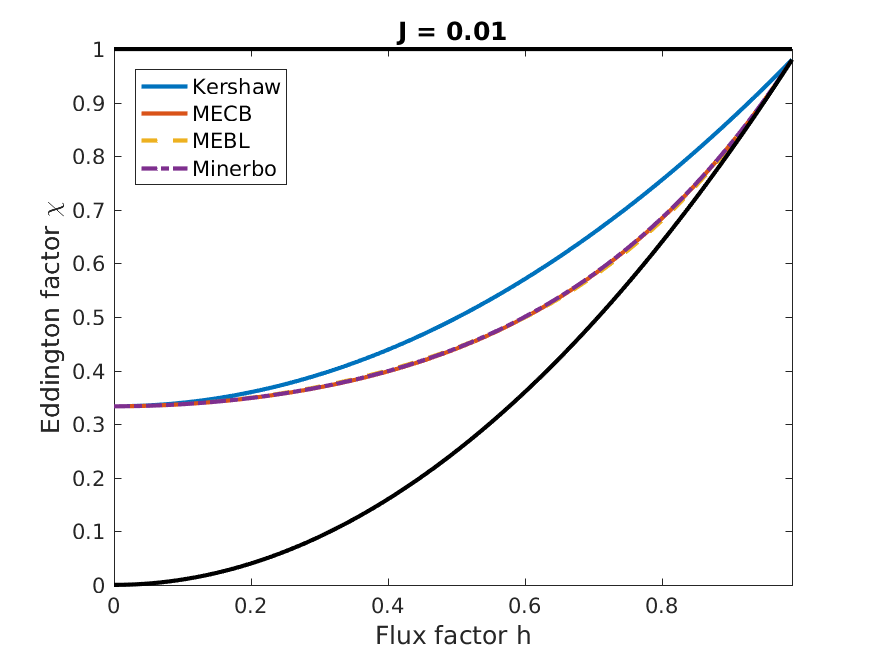
\includegraphics[width=0.5\textwidth]{figures/Closures0_01}
    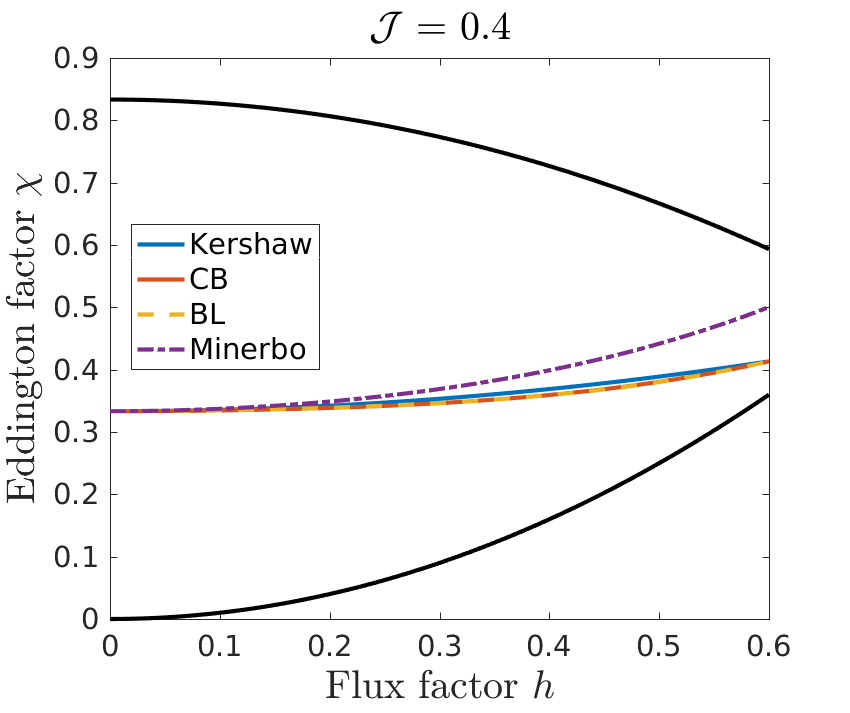
\includegraphics[width=0.5\textwidth]{figures/Closures0_40} \\
    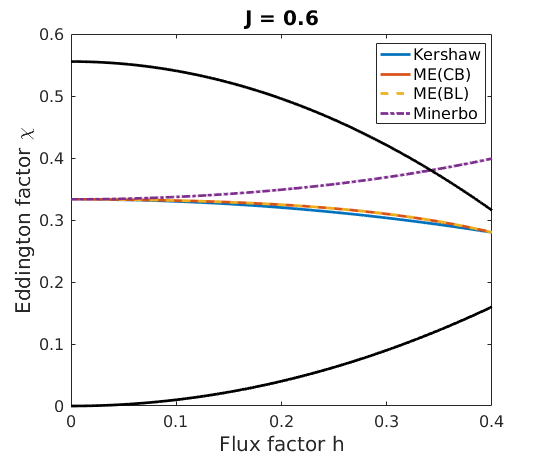
\includegraphics[width=0.5\textwidth]{figures/Closures0_60}
    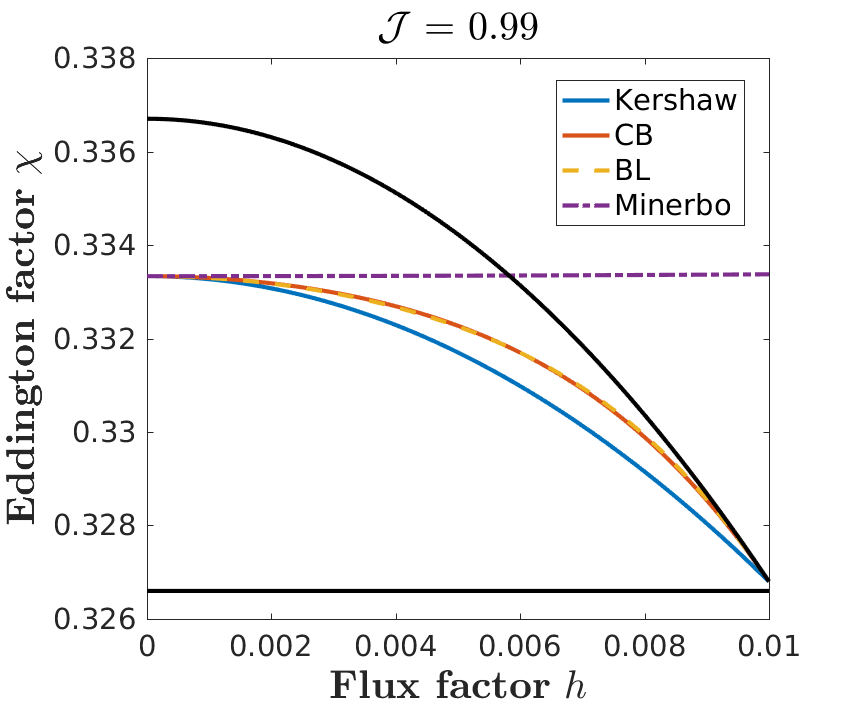
\includegraphics[width=0.5\textwidth]{figures/Closures0_99}
  \end{tabular}
   \caption{Plot of Eddington factors $\chi$ versus flux factor $h$ for different values of $\cJ$ for various algebraic closures: $\cJ=0.01$ (upper left panel), $\cJ=0.4$ (upper right panel), $\cJ=0.6$ (lower left panel), and $\cJ=0.99$ (lower right panel).  In each panel we plot the Eddington factors of Kershaw (solid blue lines), Cernohorsky \& Bludman (CB, solid red lines), Banach \& Larecki (BL, dashed orange lines), and Minerbo (dash-dot purple lines).  We also plot $\chi_{\mbox{\tiny min}}$ and $\chi_{\mbox{\tiny max}}$ defined in Eq.~\eqref{eq:eddingtonFactorBounds} (lower and upper solid black lines, respectively).}
  \label{fig:EddingtonFactorsWithDifferentClosure}
\end{figure}
We have also checked numerically that for all the algebraic closures based on Fermi-Dirac statistics (CB, BL, and Kershaw), the bounds on the Eddington factor in Eq.~\eqref{eq:eddingtonFactorBounds} holds for all $\vect{\cM}\in\cR$.  
Thus, we conclude that these closures are suited for development of realizability-preserving numerical methods for the two-moment model of fermion transport.  

In Figure~\ref{fig:MabWithDifferentClosure}, we further illustrate properties of the algebraic closures by plotting $\vect{\cM}_{ab}$ as defined in Lemma~\ref{lem:explicitStep} for the maximum entropy closures of CB and Minerbo.  
In both panels, we plot $\vect{\cM}_{ab}$ constructed from randomly selected pairs $\vect{\cM}_{a},\vect{\cM}_{b}\in\cR$ (each blue dot represents one realization of $\vect{\cM}_{ab}$).  
Results for the maximum entropy closure of CB are plotted in the left panel, while results for the Minerbo closure are plotted in the right panel.  
As expected for the closure consistent with moments of Fermi-Dirac distributions (CB), we find $\vect{\cM}_{ab}\in\cR$.  
For the Minerbo closure, which is consistent with positive distributions, $\vect{\cM}_{ab}$ is not confined to $\cR$.  
\begin{figure}[H]
  \centering
  \begin{tabular}{cc}
%    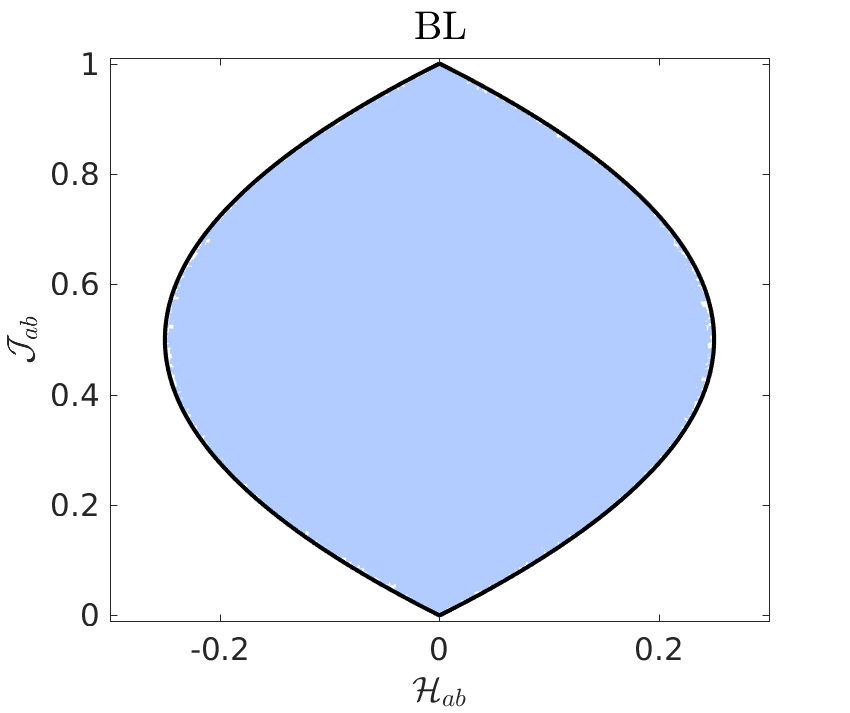
\includegraphics[width=0.5\textwidth]{figures/MabWithBLME}
    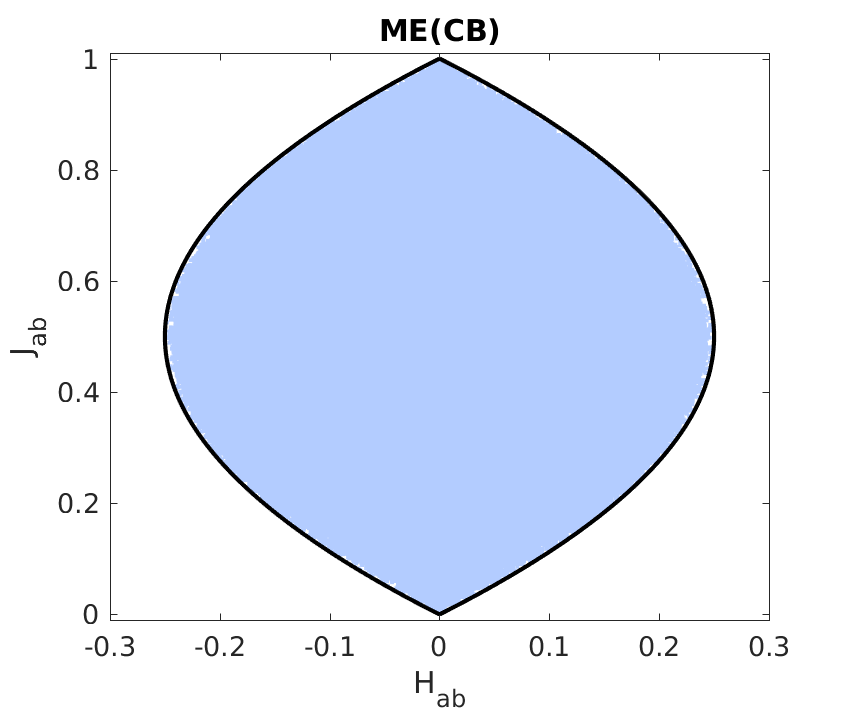
\includegraphics[width=0.5\textwidth]{figures/MabWithCBME}
%    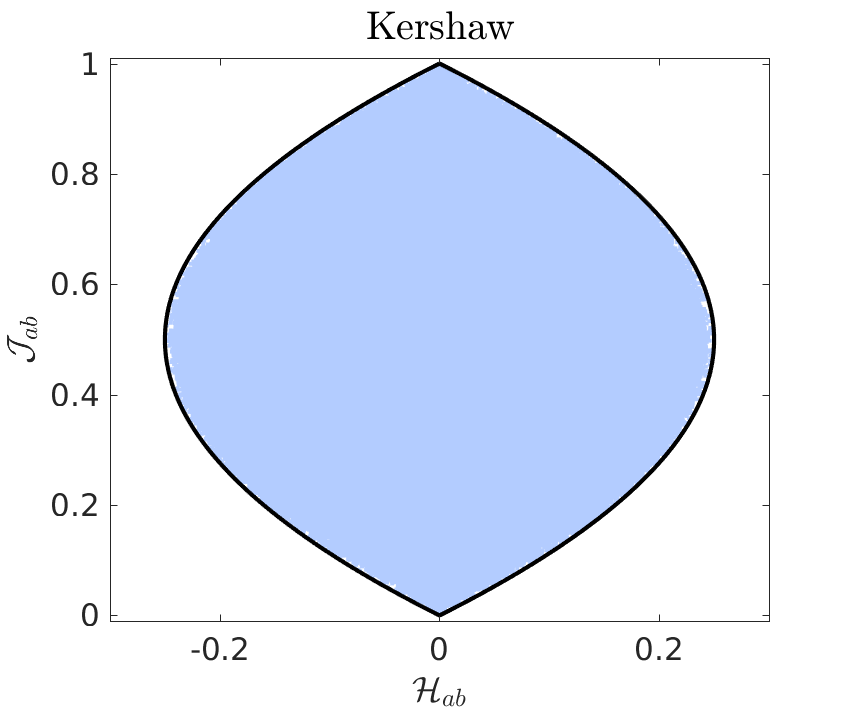
\includegraphics[width=0.5\textwidth]{figures/MabWithBLKS}
    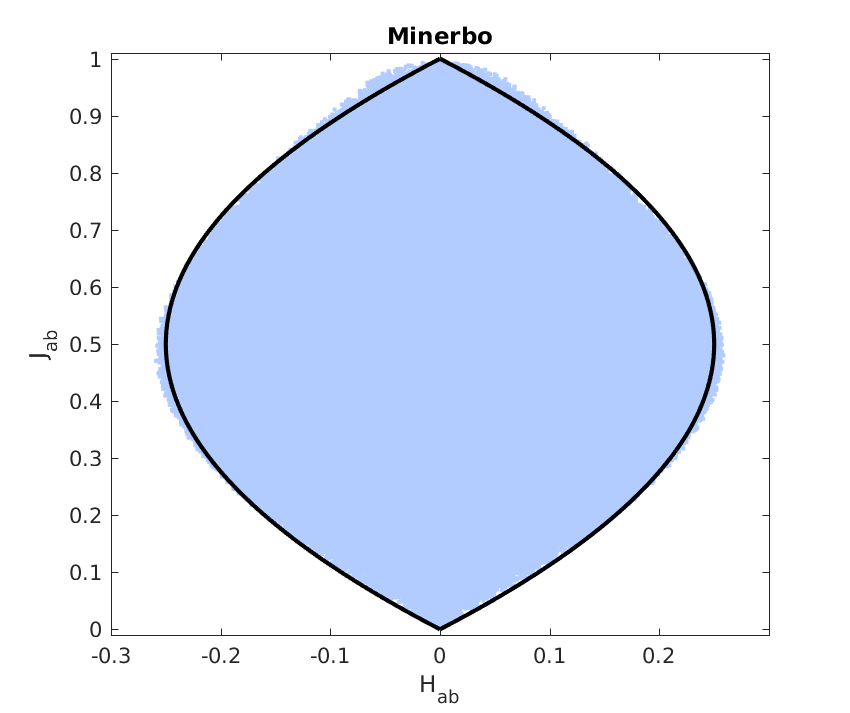
\includegraphics[width=0.5\textwidth]{figures/MabWithMI}
  \end{tabular}
   \caption{Illustration of $\vect{\cM}_{ab}$, as defined in Lemma~\ref{lem:explicitStep}, computed with algebraic maximum entropy closures of Cernohorsky \& Bludman (left) and Minerbo (right).  In each panel, $\vect{\cM}_{ab}$ was computed using the respective closure, using $10^{6}$ random pairs ($\vect{\cM}_{a},\vect{\cM}_{b}\in\cR$), and plotted as a light-blue point.  The solid black lines mark the boundary of $\cR$: $\gamma(\vect{\cM}) = 0$.}
  \label{fig:MabWithDifferentClosure}
\end{figure}